\documentclass{beamer}

\usepackage[utf8]{inputenc} % Language and font encoding
\usepackage[icelandic]{babel}
\usepackage[T1]{fontenc}


\usepackage{tikz}
\usepackage[listings,theorems]{tcolorbox}
\usepackage{booktabs}
\usepackage{minted} %Minted and configuration
\usemintedstyle{default}

\renewcommand{\theFancyVerbLine}{\sffamily \arabic{FancyVerbLine}}
%%%%%%%%%%%
% More math
%%%%%%%%%%%
\newcommand{\Mod}[1]{\ \text{mod}\ #1}

%%%%%%%%%%%%%%%%%%%%%%
% Beamer configuration
%%%%%%%%%%%%%%%%%%%%%%
\setbeamertemplate{navigation symbols}{}
\usecolortheme{dove}
\setbeamercolor{frametitle}{fg=white}

\usebackgroundtemplate%
{%
\vbox to \paperheight{

\includegraphics[width=\paperwidth]{Pics/hi-slide-head-2016}

\vfill
\hspace{0.5cm}
\includegraphics[width=0.3\paperwidth]{Pics/hi-von-logo}
\vspace{0.4cm}
    }%
}

\AtBeginSection[]
{
  \begin{frame}<beamer>
    \frametitle{Yfirlit}
    \tableofcontents[currentsection]
  \end{frame}
}

\setbeamerfont{frametitle}{size=\normalsize}
\addtobeamertemplate{frametitle}{}{\vspace*{0.5cm}}

%%%%%%%%%%%%%%%%%%%%%%%%%
% tcolorbox configuration
%%%%%%%%%%%%%%%%%%%%%%%%%

% Setup from: http://tex.stackexchange.com/a/43329/21638
\tcbset{%
    noparskip,
    colback=gray!10, %background color of the box
    colframe=gray!40, %color of frame and title background
    coltext=black, %color of body text
    coltitle=black, %color of title text 
    fonttitle=\bfseries,
    alerted/.style={coltitle=red, colframe=gray!40},
    example/.style={coltitle=black, colframe=green!20, colback=green!5},
}


%%%%%%%%%%%%%%%%%%%%%%%
% Further configuration
%%%%%%%%%%%%%%%%%%%%%%%
\hypersetup{colorlinks=true,pdfauthor={Eirikur Ernir Thorsteinsson},linkcolor=blue,urlcolor=blue}
\graphicspath{{./Pics/}}

\author{Eiríkur Ernir Þorsteinsson}
\institute{Háskóli Íslands}
\date{Haust 2016}

\title{Stærðfræðimynstur í tölvunarfræði}
\subtitle{Vika 2, fyrri fyrirlestur}

\begin{document}

\begin{frame}
\titlepage
\end{frame}

\section{Inngangur}

\begin{frame}{Í síðasta tíma}
\begin{itemize}
 \item Skoðuðum hagnýtingar á yrðingum
 \item Sáum staðalsnið fyrir yrðingar
 \begin{itemize}
  \item Eð-að staðalsnið
  \item Og-að staðalsnið
 \end{itemize}
 \item Kynntumst umsögnum
 \item Kynntumst mögnurum
\end{itemize}
\end{frame}

\section{Mengi}

\begin{frame}{Mengi}
\begin{itemize}
 \item Mengi (e. \emph{set}) er grundvallareining í strjálli stærðfræði
 \item Skyld hugmynd ``hópur'':
 \begin{itemize}
  \item Mengi eru notuð til að ``hópa'' hluti saman
  \item ``Hópur'' af hlutum myndar mengi
 \end{itemize}
 \item ``Hlutur'' í mengi er kallaður stak (e. \emph{member} eða \emph{element})
 \item Hlutir í sama mengi eiga oftast eitthvað sameiginlegt
 \item Dæmi um mengi: Allar heiltölur, allir nemendur í þessu námskeiði
\end{itemize}
\end{frame}

\begin{frame}{Skilgreining á mengi}

Klassísk skilgreining á mengi er eftirfarandi:
\begin{tcolorbox}[title=Mengi]
Mengi er óraðað samansafn hluta. Hlutur í mengi er kallaður stak þess. Mengi inniheldur stök sín. $a \in A$ táknar að stakið $a$ sé í menginu $A$. $a \notin A$ táknar að $a$ sé ekki í $A$.
\end{tcolorbox}

\end{frame}

\begin{frame}{Að tilgreina mengi}
\begin{itemize}
 \item Slaufusvigar eru oftast notaðir til að afmarka mengi
 \item Nokkrar leiðir eru algengar þegar kemur að því að tilgreina stök mengis
 \begin{itemize}
  \item Að telja upp öll stökin: 
  \begin{itemize}
   \item Mengi enskra sérhljóða: $\{a, e, i, o, u\}$ \pause
  \end{itemize}
  \item Að sýna mynstur og láta þrípunkt tákna ``augljósa'' endurtekningu:
  \begin{itemize}
   \item Mengi jákvæðra heiltalna minni en 100: $\{1, 2, 3,\ldots, 100\}$ \pause
  \end{itemize}
  \item Að tilgreina skilyrði sem stök þurfa að uppfylla:
  \begin{itemize}
   \item $\{x \in \mathbf{Z^+} | x < 100\}$ \pause
  \end{itemize}
 \end{itemize}
 \item Sum mengi hafa stöðluð nöfn: $\mathbf{R}$ (mengi rauntalna), $\mathbf{Z^+}$ (mengi jákvæðra heiltalna), \ldots
\end{itemize}
\end{frame}

\begin{frame}{Hvað má fara í mengi?}
\begin{itemize}
 \item Skilgreiningin okkar á mengjum leyfir ýmislegt
 \begin{itemize}
  \item Mengi af mengjum: $\{\mathbf{N}, \mathbf{Z}, \mathbf{Q}, \mathbf{R}\}$
 \end{itemize}
 \item Tómt mengi, táknað $\emptyset$
 \begin{itemize}
  \item Mengi sem inniheldur tóma mengið $\{\emptyset\}$
 \end{itemize}
 \item Þessi opna skilgreining veldur tæknilegum vandræðum
\end{itemize}
\end{frame}

\begin{frame}{Vandræði}
\begin{itemize}
 \item Látum $S$ vera mengið sem inniheldur þau mengi $x$ sem ekki innihalda sig sjálf, þ.e.a.s.
\end{itemize}
\[
 S = \{x | x \notin x\}
\]
\begin{itemize}
 \item Er $S$ í sjálfu sér? \pause
 \begin{itemize}
  \item Ef já, þá verður það að uppfylla það skilyrði að vera ekki í sjálfu sér \pause
  \item Ef nei, þá uppfyllir það skilyrðið sem það þarf að uppfylla til að vera í sjálfu sér \pause
 \end{itemize}
 \item Þversögn. Leiddi til frumsendulegrar mengjafræði (e. \emph{axiomatic set theory}), sem er strangari
 \begin{itemize}
  \item Þversögnin er kennd við Russell, Russell's Paradox
 \end{itemize}

\end{itemize}
\end{frame}

\section{Skilgreiningar sem tengjast mengjum}

\begin{frame}{Jöfn mengi}
\begin{tcolorbox}[title=Jöfn mengi]
Tvö mengi eru jöfn (e. \emph{equal}) ef þau innihalda sömu stök, þ.e.a.s. $\forall x (x \in A \leftrightarrow x \in B ) $. Við skrifum $A = B$ ef mengin $A$ og $B$ eru jöfn.
\end{tcolorbox}
Til dæmis eru mengin $\{a, b, c\}$ og $\{b, c, a\}$ jöfn. Sömuleiðis $\{a, b, c\}$ og $\{a, a, b, c\}$.
\end{frame}

\begin{frame}{Hlutmengi}
\begin{tcolorbox}[title=Hlutmengi]
Mengið $A$ er hlutmengi í (e. \emph{subset of}) $B$ þá og því aðeins að hvert stak í $A$ sé einnig í $B$, þ.e.a.s. $\forall x (x \in A \to x \in B)$. Við skrifum $A \subseteq B$ ef $A$ er hlutmengi í $B$.
\end{tcolorbox}

Athugum að séu tvö mengi jöfn, þá er $A \subseteq B$ og $B \subseteq A$.
\end{frame}

\begin{frame}{Tóma mengið sem hlutmengi}
\begin{itemize}
 \item Er tóma mengið hlutmengi í öllum mengjum? \pause
 \item Athugum skilgreininguna:
 \begin{itemize}
  \item Látum $S$ vera mengi. Gildir $\forall x (x \in \emptyset \to x \in S)$? \pause
  \item $x \in \emptyset$ er alltaf ósatt \pause
  \item $p \to q$ er alltaf satt þegar $p$ er ósatt
 \end{itemize}
\end{itemize}
\end{frame}

\begin{frame}{Fjöldatala mengis}
\begin{tcolorbox}[title=Fjöldatala]
Látum $S$ vera mengi. Séu $n$ mismunandi stök í $S$ og $n \in \mathbf{Z^+}$, þá er $S$ endanlegt mengi (e. \emph{finite set}) og $n$ er fjöldatala (e. \emph{cardinality}) mengisins $S$. Fjöldatala (eða stærð) mengisins $S$ er táknuð með $|S|$.
\end{tcolorbox}
Hægt er að skilgreina fjöldatölur fyrir mengi sem eru ekki endanleg.
\end{frame}

\begin{frame}{Veldismengi mengis}
\begin{tcolorbox}[title=Veldismengi]
Látum $S$ vera mengi. Þá er veldismengi (e. \emph{power set}) $S$ mengi allra hlutmengja $S$. Veldismengi $S$ er táknað með $\mathbf{P}(S)$.
\end{tcolorbox}
Dæmi: \[\mathbf{P}(\{0, 1\}) = \pause \{\emptyset, \{0\}, \{1\}, \{0, 1\}\}\]

Athugum að tóma mengið og mengið sjálft eru alltaf stök í veldismengi mengis.
\end{frame}

\begin{frame}{Mengjamargfeldi}
\begin{tcolorbox}[title=Mengjamargfeldi]
Látum $A$ og $B$ vera mengi. Mengjamargfeldi $A$ og $B$ er mengi allra raðaðra para $(a, b)$ þar sem $a \in A$ og $b \in B$, þ.e.a.s. mengið $\{(a, b) | a \in A \land b \in B\}$. Mengjamargfeldi $A$ og $B$ er táknað með $A \times B$.
\end{tcolorbox}
Dæmi:
\[
 \{1, 2\} \times \{a, b\} = \pause \{(1, a), (1, b), (2, a), (2, b)\}
\]
Athugum að almennt gildir ekki að $A \times B$ sé jafnt $B \times A$.
\end{frame}

\begin{frame}{Sammengi}
\begin{tcolorbox}[title=Sammengi]
Látum $A$ og $B$ vera mengi. 
Sammengi (e. \emph{union}) mengjanna er mengið sem inniheldur stökin sem eru í $A$ eða $B$, 
þ.e.a.s. mengið $\{x | x \in A \lor x \in B \}$. 
Sammengi $A$ og $B$ er táknað með $A\cup B$.
\end{tcolorbox}
Dæmi:
\[
 \{1, 3\} \cup \{1, 2, 4\} = \pause \{1, 2, 3, 4\}
\]
\end{frame}

\begin{frame}{Sniðmengi}
\begin{tcolorbox}[title=Sniðmengi]
Látum $A$ og $B$ vera mengi.
Sniðmengi (e. \emph{intersection}) mengjanna er mengið sem inniheldur stökin sem eru í $A$ og $B$, 
þ.e.a.s. mengið $\{x | x \in A \land x \in B \}$. 
Sniðmengi $A$ og $B$ er táknað með $A\cap B$.
\end{tcolorbox}
Mengi eru kölluð sundurlæg (e. \emph{disjoint}) ef sniðmengi þeirra er tóma mengið.

Dæmi um sniðmengi:
\[
 \{1, 3\} \cap \{1, 2, 4\} = \pause \{1\}
\]
\end{frame}

\begin{frame}{Mengjamismunur}
\begin{tcolorbox}[title=Mengjamismunur]
Mismunur mengjanna $A$ og $B$ er mengi þeirra staka sem eru í $A$ en ekki í $B$, þ.e.a.s. mengið $\{x | x \in A \land x \notin B\}$.
Mengjamismunur $A$ og $B$ er táknaður með $A - B$ eða $A \setminus B$.
\end{tcolorbox}
\end{frame}

\begin{frame}{Almengi og fyllimengi}
Fyrir mengi er hægt að skilgreina mengi allra mögulegra staka, kallað almengi (e. \emph{universal set}) oft táknað með $U$. Þá má skilgreina:

\begin{tcolorbox}[title=Fyllimengi]
Látum $A$ vera mengi og $U$ almengi þess. Þá er fyllimengi $A$ m.t.t. $U$ mengið $U \setminus A$. Fyllimengi $A$ er táknað með $\overline{A}$.
\end{tcolorbox}

Algengt er að nefnd mengi á borð við $\mathbf{R}$ eða $\mathbf{N}$ þjóni sem almengi.
\end{frame}

\section{Mengjajafngildi}

\begin{frame}{Mengjajafngildi}
\begin{columns}
\column{0.3\textwidth}
Með þessum skilgreiningum má rökstyðja ýmis jafngildi fyrir mengi.

\vspace*{0.5cm}
Tafla úr kafla 2.2.
\column{0.7\textwidth}
\begin{center}
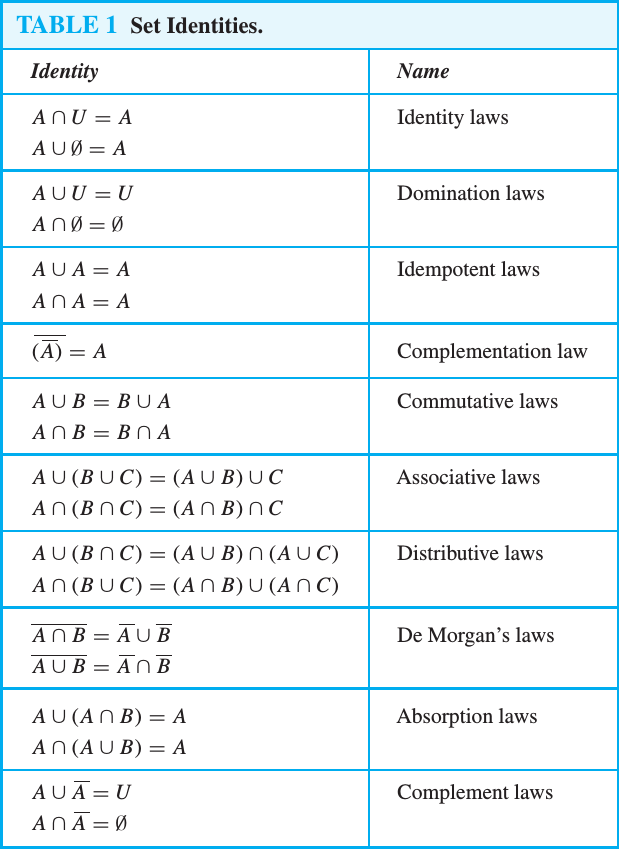
\includegraphics[height=0.8\textheight]{set-equivalences}
\end{center}
\end{columns}
\end{frame}

\begin{frame}{Útleiðsla á De Morgan fyrir mengi}
Viljum sýna að $\overline{A \cap B} = \overline{A} \cup \overline{B}$.

\begin{align*}
\overline{A \cap B} &= \{x | x \notin A \cap B\}\\ 
&= \{x | \lnot ( x \in A \cap B)\}\\ 
&= \{x | \lnot ( x \in A \land x \in B)\}\\ 
&= \{x | \lnot ( x \in A) \lor \lnot (x \in B)\}\\ 
&= \{x | x \notin A \lor x \notin B\}\\ 
&= \{x | x \in \overline{A} \lor x \in \overline{B}\}\\ 
&= \{x | x \in \overline{A} \cup \overline{B}\}\\ 
&= \overline{A} \cup \overline{B}
\end{align*}
\end{frame}

\begin{frame}{Meðlimatöflur}
Hægt er að kanna jafngildi með meðlimatöflu, sem svipar til sanntöflu:
\begin{center}
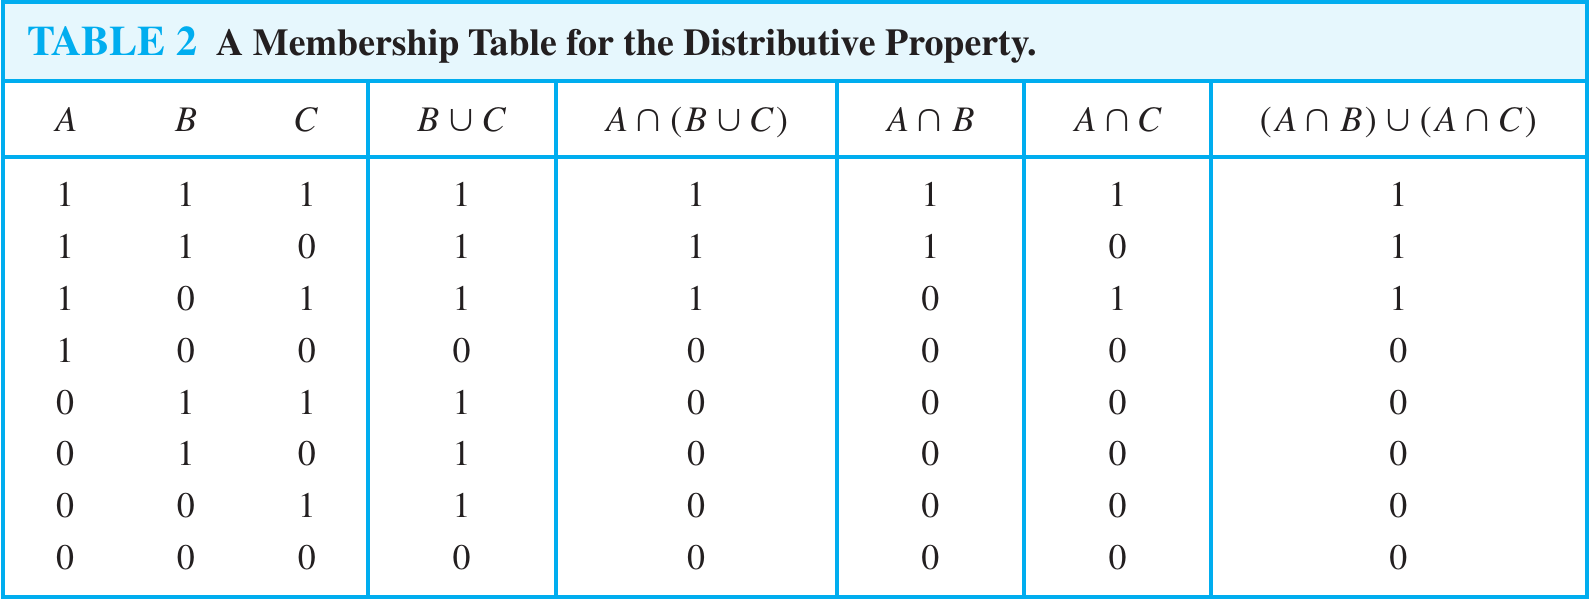
\includegraphics[width=\textwidth]{membership-table}
\end{center}
\end{frame}

\begin{frame}{Útvíkkun}
Sammengi margra mengja er mengi þeirra staka sem er í a.m.k. einu mengjanna:
\[
 A_1 \cup A_2 \cup \ldots \cup A_n = \bigcup_{i=1}^n A_i
\]
Sniðmengi margra mengja er mengi þeirra staka sem er í öllum mengjunum:
\[
 B_1 \cap B_2 \cap \ldots \cap B_n = \bigcap_{i=1}^n B_i
\]
\end{frame}

\section{Mengi í tölvum}

\begin{frame}[fragile]{Gagnagerðir sem mengi}
 \begin{itemize}
  \item Hugmyndin um gagnagerð (e. \emph{data type}) byggir á mengjum
  \item Gagnagerð samanstendur af mengi mögulegra gilda og aðgerðum á þau
  \item Gagnagerðin \texttt{Boolean} í Java skilgreinist af:
  \begin{itemize}
   \item Menginu \{\texttt{true},\texttt{false}\}
   \item Aðgerðum: Og (\verb|&&|), eða (\verb&||&), \ldots
  \end{itemize}
 \end{itemize}
\end{frame}

\begin{frame}[fragile]{Tölvuframsetning á mengjum}
Hægt er að tákna mengi með bitastrengjum.

Gerum ráð fyrir að $U$ hafi fjöldatöluna $n$ og skilgreinum fyrir það röðun. Setjum stök þess í rununa $a_1, a_2, \ldots a_n$.

Táknum þá hlutmengi $A$ í $U$ með því að að nota $n$ bita runu, þar sem $i$-ti bitinn er 1 sé $a_i$ í $A$, annars 0.
\end{frame}

\begin{frame}[fragile]{Dæmi um bitaframsetningu}
Látum $U = \{1, 2, 3, 4, 5, 6, 7, 8, 9, 10\}$. Þá er mengi oddatalna í $U$ mengið $\{1, 3, 5, 7, 9\}$, sem við getum táknað með bitarununni $1010101010$. 

Getum séð að fyllimengi oddatalnanna er $0101010101$. Hægt er að nota bitaaðferðir til að reikna út sniðmengi og sammengi.
\end{frame}

\begin{frame}{Næst}
Föll (kafli 2.3), rakningavensl (kafli 2.4), reiknanleiki (kafli 2.5), fylki (kafli 2.6)
\end{frame}


\end{document}
